\begin{wrapstuff}[r,leftsep=0.75em,rightsep=0.75em,top=1]
	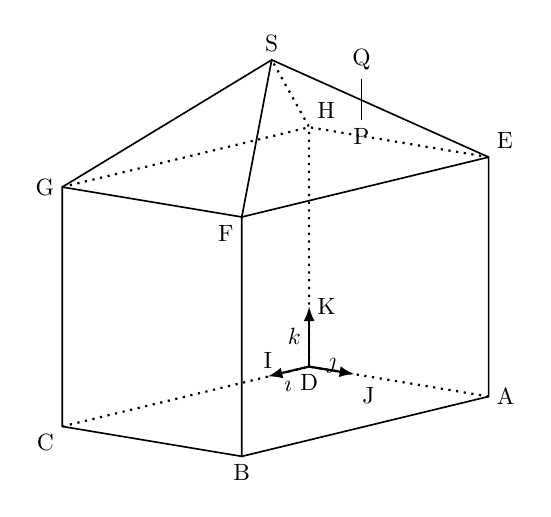
\begin{tikzpicture}[scale=0.95,every node/.style={scale=0.85}]
		\draw[semithick] (0.3,3.9)--(0.3,0.7)--(2.7,0.3)--(2.7,3.5)--cycle;%GCBF
		\draw[semithick] (2.7,0.3)--(6,1.1)--(6,4.3)--(2.7,3.5);%BAEF
		\draw[thick,dotted] (0.3,0.7)--(3.6,1.5)--(6,1.1);%CDA
		\draw[thick,dotted] (3.6,1.5)--(3.6,4.7)--(3.1,5.6);%DHS
		\draw[thick,dotted] (0.3,3.9)--(3.6,4.7)--(6,4.3);%GHE
		\draw[semithick] (6,4.3)--(3.1,5.6)--(2.7,3.5);%ESF
		\draw[semithick] (3.1,5.6)--(0.3,3.9);%SG
		\draw[semithick] (4.3,4.8)--(4.3,5.35);%PQ
		\draw[thick,->,>=latex] (3.6,1.5)--(3.05,1.37);
		\draw[thick,->,>=latex] (3.6,1.5)--(4.2,1.4);
		\draw[thick,->,>=latex] (3.6,1.5)--(3.6,2.3);
		%labels
		\draw(6,1.1) node[right] {A} ;
		\draw(2.7,0.3) node[below] {B} ;
		\draw(0.3,0.7) node[below left] {C} ;
		\draw(3.6,1.5) node[below] {D} ;
		\draw(6,4.3) node[above right] {E} ;
		\draw(2.7,3.5) node[below left] {F} ;
		\draw(0.3,3.9) node[left] {G} ;
		\draw(3.6,4.7) node[above right] {H} ;
		\draw(3.1,5.6) node[above] {S} ;
		\draw(4.3,4.8) node[below] {P} ;
		\draw(4.3,5.35) node[above] {Q} ;
		\draw(3.05,1.37) node[above] {I} ;
		\draw(4.2,0.9) node[above right] {J} ;
		\draw(3.6,2.3) node[right] {K} ;
		\draw(3.32,1.42) node[below] {$\vect{\imath}$} ;
		\draw(3.9,1.3) node[above] {$\vect{\jmath}$} ;
		\draw(3.6,1.9) node[left] {$\vect{k}$} ;
	\end{tikzpicture}
\end{wrapstuff}

Une maison est modélisée par un parallélépipède rectangle $ABCDEFGH$ surmonté d'une pyramide $EFGHS$.

On a $DC = 6$, $DA = DH = 4$. 

Soient les points $I$, $J$ et $K$ tels que :

\medskip

\hfill$\vect{DI} = \dfrac16\vect{DA}$ ; $\vect{DJ} = \dfrac14\vect{DA}$ et $\vect{DK} = \dfrac14\vect{DH}$.\hfill~

\medskip

On note $\vect{\imath} = \vect{DI}$, $\vect{\jmath} = \vect{DJ}$ et $\vect{k} = \vect{DK}$.

On se place dans le repère orthonormé $\left(D;\vect{\imath},\,\vect{\jmath},\, \vect{k}\right)$.

On admet que le point $S$ a pour coordonnées $(3;2;6)$.

\begin{enumerate}
	\item Donner, sans justifier, les coordonnées des points $B$, $E$, $F$ et $G$.
	\item Démontrer que le volume de la pyramide $EFGHS$ représente le septième du volume total de la maison.
	
	On rappelle que le volume $\mathcal{V}$ d'un tétraèdre est donné par la formule : \[\mathcal{V} = \dfrac13 \times (\text{aire de la base}) \times  \text{hauteur}.\]
	\item 
	\begin{enumerate}
		\item Démontrer que le vecteur $\vect{n}$ de coordonnées $\begin{pmatrix}0\\1\\1\end{pmatrix}$ est normal au plan $(EFS)$.
		\item En déduire qu'une équation cartésienne du plan $(EFS)$ est $y + z - 8 = 0$.
	\end{enumerate}
	\item On installe une antenne sur le toit, représentée par le segment $[PQ]$. On dispose des données suivantes :
	
	\begin{itemize}
		\item le point $P$ appartient au plan $(EFS)$ ;
		\item le point $Q$ a pour coordonnées $(2;3;5,5)$ ;
		\item la droite $(PQ)$ est dirigée par le vecteur $\vect{k}$.
	\end{itemize}
	\begin{enumerate}
		\item Justifier qu'une représentation paramétrique de la droite $(PQ)$ est : \[ \begin{dcases}  x=2 \\ y = 3 \\ z=5,5+t \end{dcases} \quad (t \in \R).\]
		\item En déduire les coordonnées du point $P$.
		\item En déduire la longueur $PQ$ de l'antenne.
		
		Un oiseau vole en suivant une trajectoire modélisée par la droite $\Delta$ dont une représentation paramétrique est : \[ \begin{dcases}  x=-4+6s \\ y = \phantom{-}7-4s \\ z=\phantom{-}2+4s \end{dcases} \quad (s \in \R).\]%
		Déterminer la position relative des droites (PQ) et $\Delta$.
		
		L'oiseau va-t-il percuter l'antenne représentée par le segment $[PQ]$ ?
	\end{enumerate}
\end{enumerate}

